\section{Background}\label{sec:problem}
Consider a swarm $\mathcal{N}$ of $N$ robots labelled $i\in\left\{1,...,N\right\}$. The swarm is modeled as a directed sensing graph $\mathcal{G}=\left(\mathcal{V},\mathcal{E}\right)$, where vertex set $\mathcal{V} = \left\{1,..., N\right\}$ represents the robots, and edge set $\mathcal{E}\subseteq\mathcal{V}\times \mathcal{V}$ includes robot pairs $\left(i, j\right)\in\mathcal{E}$ for which robot $i$ can sense robot $j$. Denote $\mathcal{N}_i=\left\{j\in\mathcal{V}|\left(i,j\right)\in\mathcal{E}\right\}\subset\mathcal{V}$ as the set of $N_i$ neighbours of a robot $i$ in $\mathcal{G}$.

In this work, the dynamics of the robots are represented in discrete time. Denote $p_i(k),v_i(k),u_i(k)\in\mathbb{R}^3$ respectively be the position, velocity and control input of robot $i$ at time $t(k) = k\tau$, where $\tau$ is the sampling period. The robots in the swarm are homogeneous with a body radius $r$. Each robot is equipped with an inertial measurement unit (IMU) to determine its position and orientation, a range sensor to sense the environment, and a wireless ad-hoc network module to carry out peer-to-peer communication with other robots. In this work, the communication delay between each pair of robots is negligible~\cite{AlonsoMora2018,9527169}. The range sensor provides a $360^\circ$ field of view with the scanning area $S_s$ of radius $r_s$, as shown in Fig.~\ref{fig:model}. Its data points obtained at time $t(k)$ is represented by set $\mathcal{M}_i(k)=\left\{m\right\}$.
\begin{figure}
    \centering
    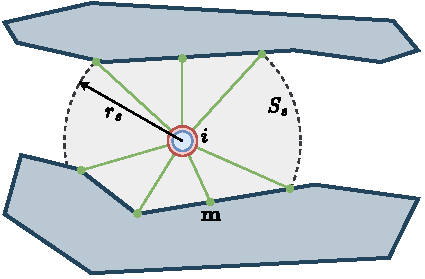
\includegraphics[width=0.48\textwidth]{paper3/images/model.pdf}
    \caption{Illustration of a robot with its range sensor having the scanning area $S_s$ (dashed gray circle) of radius $r_s$. Set $\mathcal{M}_i=\{m\}$ (green) is the observed point data.}
    \label{fig:model}
\end{figure}

According to~\cite{Soria2021}, the robot in the swarm can be represented as a discrete linear system as follows:
\begin{equation}
    x_i(k+1)=A_ix_i(k) + B_iu_i(k),
\end{equation}
where $A_i$ and $B_i$ are system matrices, $u_i$ is input acceleration, and $x_i=\left[p_i;v_i\right]\in\mathbb{R}^6$ is a state vector including position and velocity. The velocities and accelerations are bounded, i.e., $v_\text{min}\leq v_i(k)\leq v_\text{max}$ and $u_\text{min}\leq u_i(k)\leq u_\text{max}$.